\documentclass[tikz,border=10pt]{standalone}
% Scale: 1 unit = 1 cm, s = 0.021448 cm/px, origin at O
\begin{document}
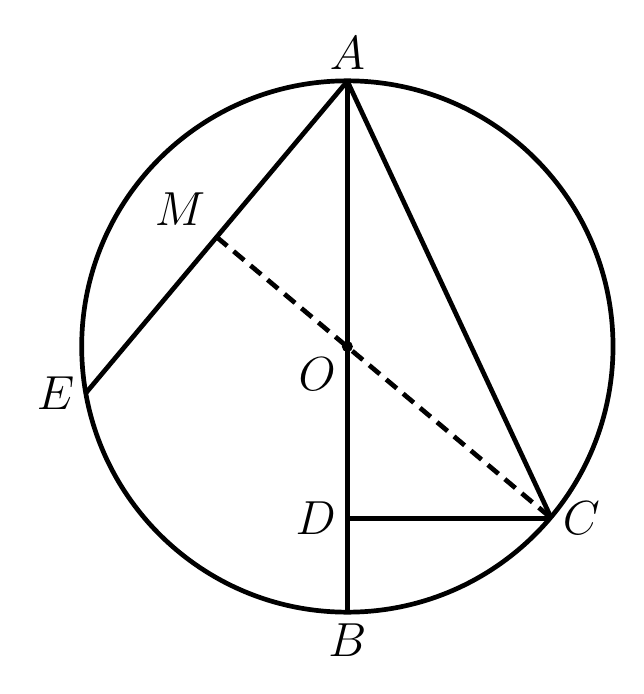
\begin{tikzpicture}[line width=1.7pt, line join=round,
    lbl/.style={font=\fontsize{17.5}{21}\selectfont}]

  % Points (converted from pixels, y flipped)
  \coordinate (O) at (0,0);
  \coordinate (A) at (0,3.37);
  \coordinate (B) at (0,-3.38);
  \coordinate (D) at (0,-2.18);
  \coordinate (C) at (2.59,-2.18);
  \coordinate (E) at (-3.32,-0.59);
  \coordinate (M) at (-1.66,1.39);

  % Circle centred at O, radius 3.37 cm
  \draw (O) circle[radius=3.374];

  % Solid segments
  \draw (A) -- (B);
  \draw (A) -- (C);
  \draw (A) -- (E);
  \draw (D) -- (C);

  % Dashed segment M--O--C (long dashes, passes through O)
  \draw[dash pattern=on 5pt off 3pt] (M) -- (C);

  % Filled dot at the centre O, drawn after the dashed path so it is on top
  \fill (O) circle (2pt);

  % Labels
  \node[lbl, above] at (A) {$A$};
  \node[lbl, below] at (B) {$B$};
  \node[lbl, right] at (C) {$C$};
  \node[lbl, left]  at (E) {$E$};
  \node[lbl, left]  at (D) {$D$};
  \node[lbl, below left] at (O) {$O$};
  \node[lbl, above left] at (M) {$M$};

\end{tikzpicture}
\end{document}